%%__________________________________________________________________||
\section{Non-multijet backgrounds}
\label{sec:ewk_background}

In the absence of multijet events, the background counts in the signal
region arise from SM processes with significant \met in the final
state. In events with low counts of jets and b-quark jets, the largest
backgrounds with genuine \met are from the associated production of W
or Z bosons with jets, followed by either the weak decays \znunu or
\wtaunu, where the $\tau$ decays hadronically and is identified as a
jet; or by leptonic decays that are not rejected by the dedicated
electron or muon vetoes. The veto of events containing isolated tracks
is efficient at further suppressing these backgrounds as well as the
single-prong hadronic decay of the tau lepton. At higher jet and
b-quark jet multiplicities, top quark production followed by
semileptonic weak top quark decay becomes important. 
%Residual contributions from processes such as single-top-quark,
%diboson, and Drell-Yan production are also expected.

The production of W and Z bosons in association with jets is simulated
with the \MADGRAPH V5~\cite{madgraph} event generator. The production
of \ttbar and single-top quark events is generated with
\POWHEG~\cite{powheg}, and diboson events are produced with
\PYTHIA6.4~\cite{pythia}. For all simulated samples, \PYTHIA6.4 is
used to describe parton showering and hadronisation. All samples are
generated using the \textsc{cteq6l1}~\cite{Pumplin:2002vw} parton
distribution functions (PDF). The description of the detector response
is implemented using the \GEANTfour~\cite{geant} package. The
simulated samples are normalised using the most accurate cross section
calculations currently available, usually with
next-to-next-to-leading-order (NNLO) accuracy. To model the effects of
pileup, the simulated events are generated with a nominal distribution
of pp interactions per bunch crossing and then reweighted to match the
pileup distribution as measured in data.

The method to estimate the non-multijet backgrounds in the signal
region relies on the use of transfer factors (TF), which are
constructed per bin (in terms of \njet, \nb, and \scalht) per data
control sample. The TFs are determined from the simulated event
samples and are ratios of expected yields in the corresponding bins of
the signal region and control samples. The TFs are used to extrapolate
from the event yields measured in a data control samples to an
expectation for the total background event yields in the signal
region. 
%Two independent estimates of the irreducible background of \znunu +
%jets events are determined from the \gj and \mmj data control samples,
%both of which have similar kinematic properties when the muons or
%photon are ignored~\cite{Bern:2011pa} but different acceptances. The
%\gj process has a larger production cross section while the \mmj
%process has kinematic properties that are more similar to $\znunu +
%\text{jets}$.

Two independent estimates of the irreducible background of \znunu +
jets events are determined from the \gj and \mmj data control samples.
The \gj and \zmumu + jets processes have similar kinematic properties
when the photon or muons are ignored~\cite{Bern:2011pa} albeit
different acceptances. In addition, the \gj process has a larger
production cross section than \znunu + jets events.

The \mj data sample provides an estimate for the total
contribution from all other SM processes, which is dominated by \ttbar
and W-boson production. Residual contributions from processes such as
single-top-quark, diboson, and Drell-Yan production are also
estimated. For the category of events satisfying $\nb \geq 2$, in
which the contribution from $\znunu + \text{jets}$ events is
suppressed to a negligible level, the \mj sample is also used to
estimate this small contribution rather than using the statistically
limited \mmj and \gj samples. Hence, only the \mj sample is used to
estimate the total SM background for events satisfying $\nb \geq 2$,
whereas all three data control samples are used for events satisfying
$\nb \leq 1$.

%In order to maximise sensitivity to potential new physics signatures
%in final states with a high b-quark content, a method that improves
%the statistical power of the predictions from simulation, particularly
%for $n_\cPqb \ge 2$, is employed~\cite{RA1Paper2012}. The distribution
%of $n_\cPqb$ is estimated from generator-level information contained
%in the simulation, namely the number of reconstruction-level jets
%matched to underlying bottom quarks ($n_\cPqb^\text{gen}$), charm
%quarks ($n_\cPqc^\text{gen}$), and light-flavoured partons
%($n_\cPq^\text{gen}$) per event. All relevant combinations of
%$n_\cPqb^{\rm gen}$, $n_\cPqc^{\rm gen}$, and $n_{\cPq}^{\rm gen}$ are
%considered, and event counts are recorded according to the
%categorisation of events in terms of \njet and \scalht. The efficiency
%$\epsilon$ with which b-quark jets are identified and the mistag
%probabilities $f_\cPqc$ and $f_\cPq$ are also determined from
%simulation per event category, with each quantity averaged over jet
%\pt and $\eta$. Corrections are applied on a jet-by-jet basis to
%$\epsilon$, $f_\cPqc$, and $f_\cPq$ in order to match the
%corresponding measurements from data~\cite{CMS-PAS-BTV-12-001}. This
%information is sufficient to predict $n_\cPqb$ and thus also determine
%the event yield from simulation for a given event category. The event
%yields for a given b-quark jet multiplicity can be predicted with a
%higher statistical precision than obtained directly from simulation,
%particularly for events with high counts of b-quark jets, and are
%subsequently used to determine the transfer factors binned according
%to \nb (in addition to \njet and \scalht).

The uncertainty in the transfer factors derived from simulation is
probed through closure tests based on data control
samples~\cite{RA1Paper2012}. Each closure test inspects the
compatability of yields in two disjoint samples and a corresponding TF
derived from simulation. A large ensemble of tests are performed to
probe key ingredients of the simulation modelling that may introduce a
source of bias in the transfer factors.
% Thirteen categories of test,
%shown in Figure~\label{fig:closure},
%are used to identify potential biases in the simulation modelling of
%aspects such as: the \alphat and \njet variables; the relative
%composition between W + jets and top events; the reconstruction of
%b-quark jets; vector boson production; and muon or photon
%reconstruction and isolation efficiencies. The closure tests also
%probe the consistency between the \mmj and \gj samples, which are both
%used in the prediction of background events from \znunu\ + jets.

%\begin{figure*}[tbhp]
%\vspace{-0.5cm}
%  \begin{center}
%\vspace{-0.3cm}
%    \subfigure[$2 \leq {\rm n_{jet}} \leq 3$]{
%      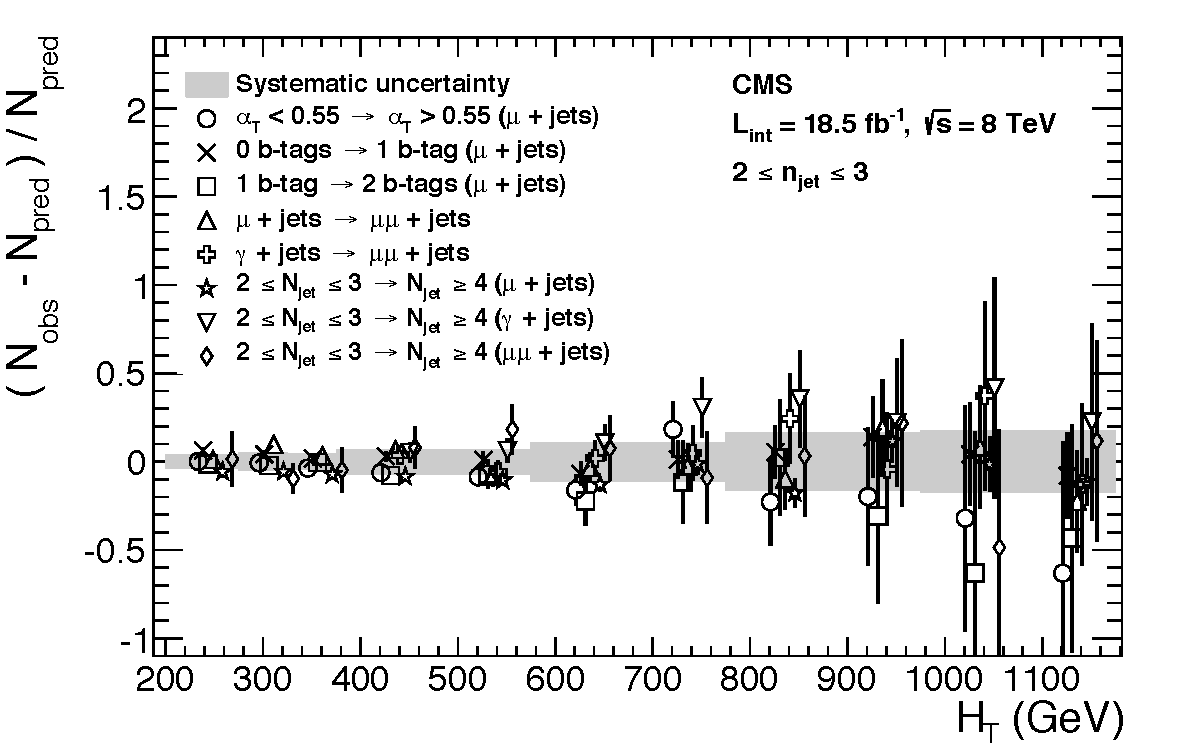
\includegraphics[width=0.505\textwidth]{figures/closure/summary_plot_njle3} 
%    }
%    \subfigure[${\rm n_{jet}}  \geq 4$]{
%      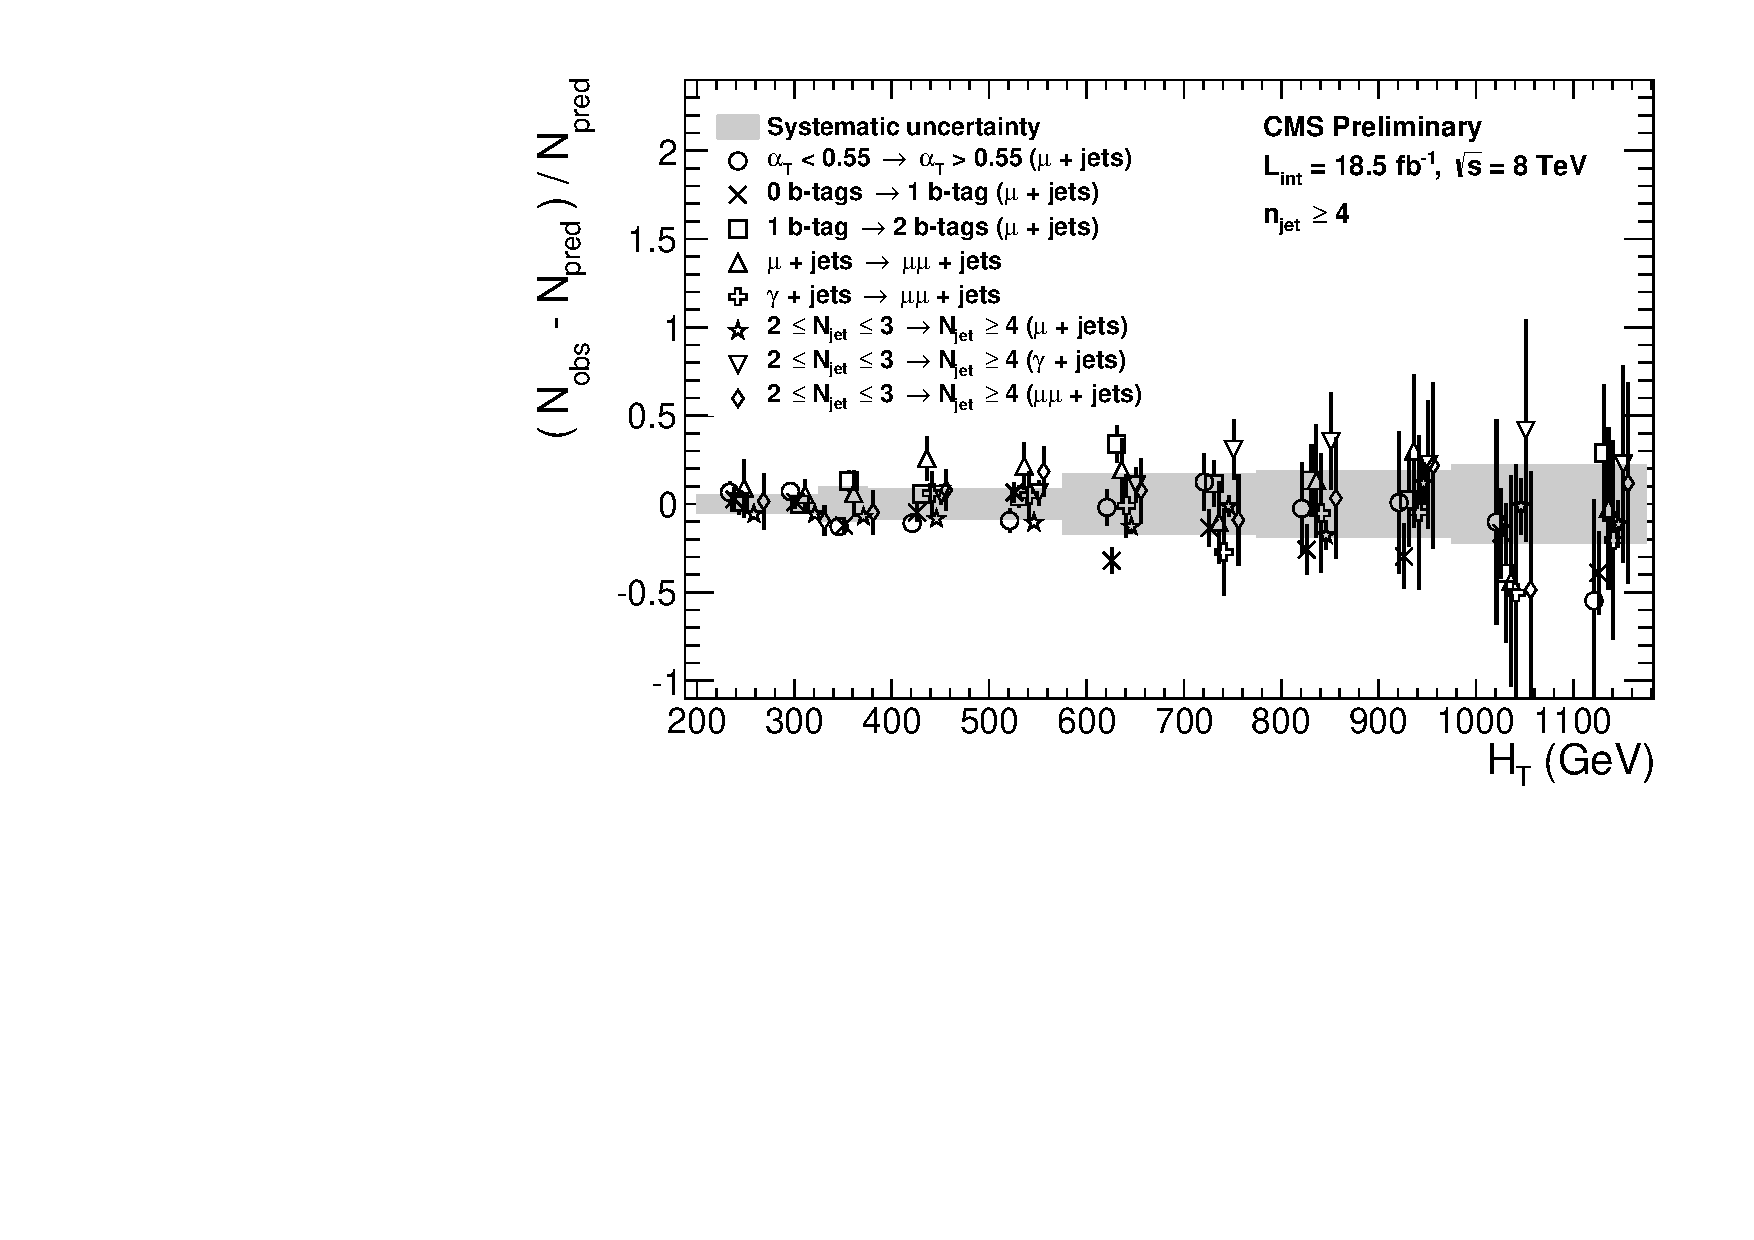
\includegraphics[width=0.505\textwidth]{figures/closure/summary_plot_njge4} 
%    } \\
%    \caption{ Sets of closure tests within and between different
%      control samples as a function of  $\scalht$ for (a) events with
%      up to three jets and (b) events with four or more jets.  \label{fig:closure} }
%  \end{center}
%\end{figure*}
%

The closure tests reveal no significant biases or dependencies on
\njet or \scalht for all individual tests. Systematic uncertainties in
the transfer factors are determined from the statistically-weighted
variance in the level of closure for collections of
tests. \FIXME{something about correlation of systematics here?}

Monte Carlo based templates are used to predict the background in the \MHT distrbution. Control regions are used to evalaute the degree to which the Monte Carlo describes the variable in data and assign appropriate systematic uncertainties.

%Uncorrelated systematic uncertainties are determined for
%regions in \scalht and each jet multiplicity category, as defined in
%Table~\ref{tab:syst-values}.  An independent study to assess the
%effect of uncertainties in the simulation modelling of the efficiency
%and mistag rates for identifying jets originating from b-quarks and
%light-flavour partons on the transfer factors is also performed and
%found to be negligible, at the sub-percent level, with respect to the
%values quoted in Table~\ref{tab:syst-values}. The same (uncorrelated)
%value of systematic uncertainty is assumed for each \nb category.

%\begin{table}[!h]
%  \caption{Systematic uncertainties (\%) in the transfer factors,
%    according to \njet and \scalht region.}
%  \label{tab:syst-values}
%  \centering
%  \footnotesize
%  \begin{tabular}{ cccccccc }
%    \hline
%    \hline
%            & \multicolumn{7}{c}{\scalht region (GeV)}                                \\
%    \cline{2-8}
%    \njet   & 200--275 & 275--325 & 325--375 & 375--575 & 575--775 & 775-975 & $>975$ \\
%    \hline                                                                                                                                  
%    2--3    & 4        & 6        & 6        & 8        & 12       & 17      & 19     \\
%    $\geq$4 & 6        & 6        & 11       & 11       & 18       & 20      & 26     \\
%    \hline                                                                                                                                  
%    \hline
%  \end{tabular}
%\end{table}

%%__________________________________________________________________||
